% Nier_ANLP -- SemEval-2026 Task 6 (CLARITY) final report.
% Built on the official ACL template (acl-org/acl-style-files @ d5adc82);
% acl.sty and acl_natbib.bst are unmodified copies. Compile with pdfLaTeX + BibTeX.
% Page budget (course rules): at most 8 pages of main text, then Limitations (not counted, placed just
% before the references), references, and at most 2 pages of appendix.
\documentclass[11pt]{article}

% "final": the camera-ready (non-anonymous) version, as the template's comment describes.
\usepackage[final]{acl}

% Standard package includes (as in the official template)
\usepackage{times}
\usepackage{latexsym}
\usepackage[T1]{fontenc}
\usepackage[utf8]{inputenc}
\usepackage{microtype}
\usepackage{inconsolata}
\usepackage{graphicx}

% Content packages (no layout changes)
\usepackage{amsmath}
\usepackage{amssymb}
\usepackage{booktabs}
\usepackage{array}
\newcolumntype{L}[1]{>{\raggedright\arraybackslash}p{#1}}
\usepackage{xurl}
\usepackage{tikz}
\usetikzlibrary{positioning,arrows.meta,fit,calc,backgrounds,shapes.geometric}

% Shared notation
\newcommand{\Stwo}{S2}
\newcommand{\Sone}{S1}
\newcommand{\pmsd}[2]{#1\,{\scriptsize$\pm$\,#2}}
\newcommand{\ci}[2]{[#1,\,#2]}
% Run-in labels that give every experiment the same shape: question, prediction, result, consequence.
\newcommand{\step}[1]{\textbf{#1}\enspace}

% Figures (data figures from code/figures/; the diagrams are TikZ)
% Figure macros. Diagrams are TikZ (figures/fig_*.tex); data figures are PDFs drawn by
% code/figures/e25_figures.py (E25_*) and code/figures/paper_figures.py via E18 (E18_frontier).

\newcommand{\FigurePath}{%
\begin{figure*}[t]
\centering
% Figure 1: the research path, five stages in one row (TikZ, monochrome). Input by \FigurePath in figs.tex.
% Box width 25.4 mm text + 2 x 1.6 mm padding; four 3.6 mm gaps: 5 x 28.6 + 4 x 3.6 = 157.4 mm (text width 160 mm).
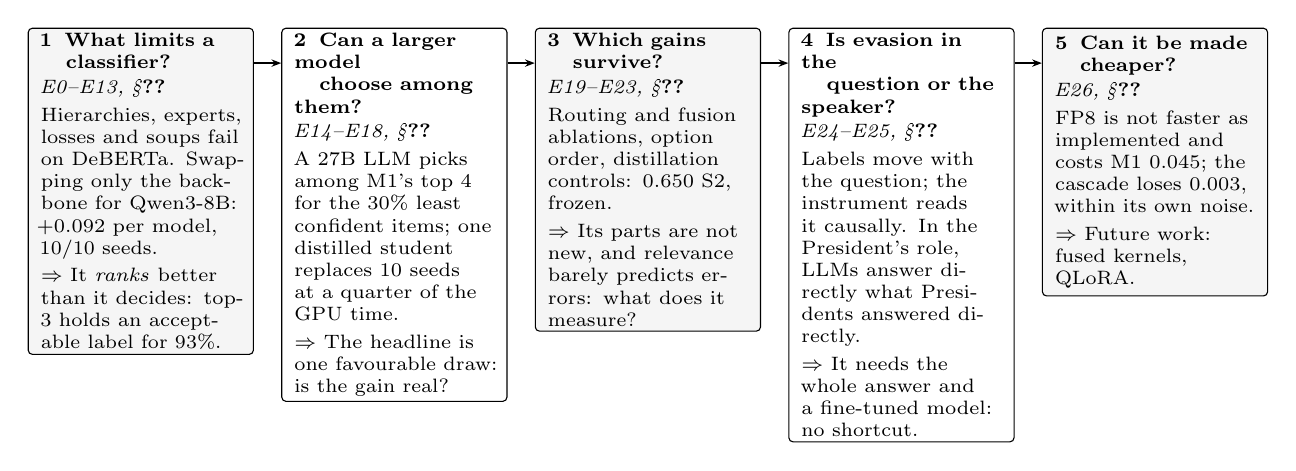
\begin{tikzpicture}[
  font=\scriptsize,
  stage/.style={draw, rounded corners=1.5pt, align=left, text width=25.4mm, inner xsep=1.6mm, inner ysep=1.8pt,
                anchor=north west, minimum height=34mm},
  arr/.style={-{Stealth[length=3.5pt]}, thick},
]
\def\gap{32.2mm}
\node[stage, fill=black!4] (s1) at (0,0) {%
  \textbf{1\enspace What limits a\\\phantom{1\enspace}classifier?}\\[1pt]
  {\itshape E0--E13, \S\ref{sec:classifier}}\\[2pt]
  Hierarchies, experts, losses and soups fail on DeBERTa. Swapping only the backbone for Qwen3-8B: +0.092 per model, 10/10 seeds.\\[2pt]
  $\Rightarrow$ It \emph{ranks} better than it decides: top-3 holds an acceptable label for 93\%.};
\node[stage] (s2) at (\gap,0) {%
  \textbf{2\enspace Can a larger model\\\phantom{2\enspace}choose among them?}\\[1pt]
  {\itshape E14--E18, \S\ref{sec:cascade}}\\[2pt]
  A 27B LLM picks among M1's top 4 for the 30\% least confident items; one distilled student replaces 10 seeds at a quarter of the GPU time.\\[2pt]
  $\Rightarrow$ The headline is one favourable draw: is the gain real?};
\node[stage, fill=black!4] (s3) at (2*\gap,0) {%
  \textbf{3\enspace Which gains\\\phantom{3\enspace}survive?}\\[1pt]
  {\itshape E19--E23, \S\ref{sec:robust}}\\[2pt]
  Routing and fusion ablations, option order, distillation controls: 0.650 \Stwo{}, frozen.\\[2pt]
  $\Rightarrow$ Its parts are not new, and relevance barely predicts errors: what does it measure?};
\node[stage] (s4) at (3*\gap,0) {%
  \textbf{4\enspace Is evasion in the\\\phantom{4\enspace}question or the speaker?}\\[1pt]
  {\itshape E24--E25, \S\ref{sec:measure}}\\[2pt]
  Labels move with the question; the instrument reads it causally. In the President's role, LLMs answer directly what Presidents answered directly.\\[2pt]
  $\Rightarrow$ It needs the whole answer and a fine-tuned model: no shortcut.};
\node[stage, fill=black!4] (s5) at (4*\gap,0) {%
  \textbf{5\enspace Can it be made\\\phantom{5\enspace}cheaper?}\\[1pt]
  {\itshape E26, \S\ref{sec:precision}}\\[2pt]
  FP8 is not faster as implemented and costs M1 0.045; the cascade loses 0.003, within its own noise.\\[2pt]
  $\Rightarrow$ Future work: fused kernels, QLoRA.};
\foreach \a/\b in {s1/s2, s2/s3, s3/s4, s4/s5}
  \draw[arr] ($(\a.north east)+(0,-4.5mm)$) -- ($(\b.north west)+(0,-4.5mm)$);
\end{tikzpicture}

\caption{The research path. Each stage answers one question, and its answer (last line of each box) raises the next. Experiment ids refer to the ledger in Appendix~\ref{sec:ledger}.}
\label{fig:path}
\end{figure*}}

\newcommand{\FigureSystem}{%
\begin{figure*}[t]
\centering
% Figure 2: the whole system in one picture (TikZ, monochrome, within the 160 mm text width). Input by \FigureSystem.
% Three columns: (left) what is trained or fitted, and on which data; (middle) the cascade, which after E23 is the
% frozen instrument; (right) how the instrument is used in E25/E26. Each side box sits level with the stage it
% feeds, so every arrow is straight. Widths: side 38 mm, middle 54 mm, gaps 7 mm (frames span ~153 mm).
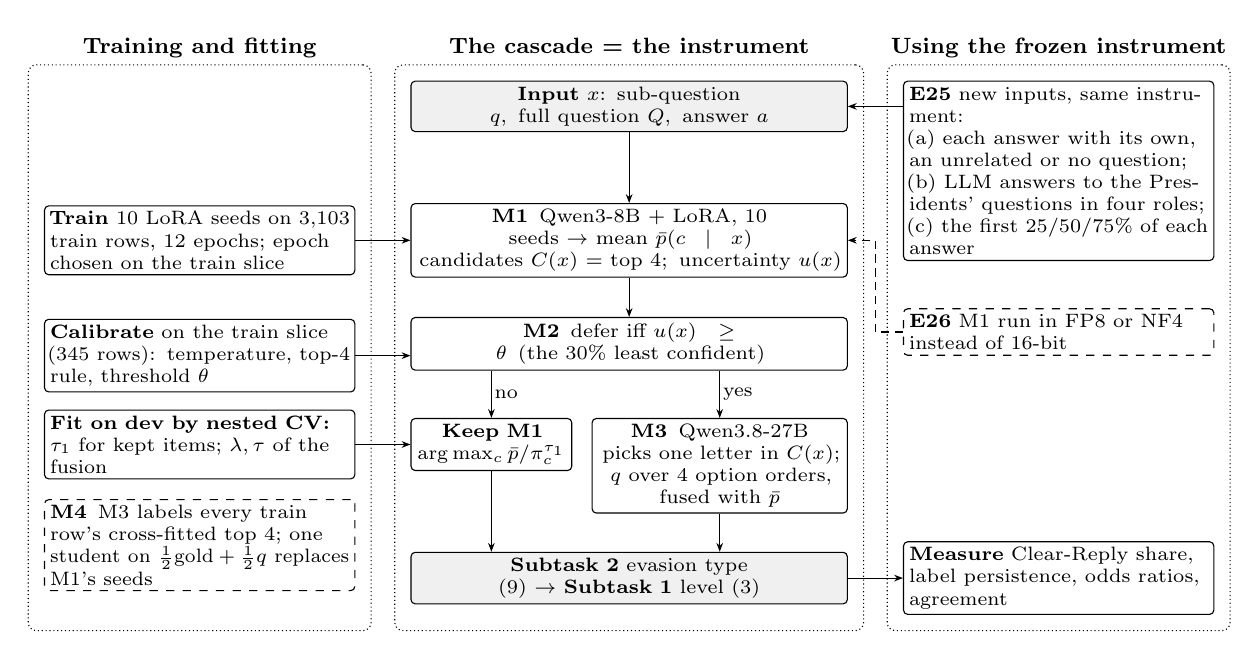
\begin{tikzpicture}[
  font=\scriptsize,
  box/.style={draw, rounded corners=1.5pt, align=center, inner xsep=2pt, inner ysep=2pt},
  side/.style={box, align=left, text width=38mm},
  arr/.style={-{Stealth[length=3.2pt]}, thin},
  head/.style={font=\footnotesize\bfseries, anchor=south, inner sep=2pt, text height=1.7ex, text depth=0.4ex},
  frame/.style={draw, densely dotted, rounded corners=3pt, inner sep=2mm},
]
% ---------------- middle column: the cascade ----------------
\node[box, fill=black!6, text width=54mm, anchor=north] (in) at (80mm,0) {%
  \textbf{Input} $x$:\enspace sub-question $q$,\enspace full question $Q$,\enspace answer $a$};
\node[box, text width=54mm, anchor=north] (m1) at ($(in.south)+(0,-9mm)$) {%
  \textbf{M1}\enspace Qwen3-8B + LoRA, 10 seeds $\rightarrow$ mean $\bar p(c \mid x)$\\
  candidates $C(x)$ = top 4;\enspace uncertainty $u(x)$};
\node[box, text width=54mm, anchor=north] (m2) at ($(m1.south)+(0,-5mm)$) {%
  \textbf{M2}\enspace defer iff $u(x) \ge \theta$\enspace(the 30\% least confident)};
\node[box, text width=19mm, anchor=north west] (keep) at ($(m2.south west)+(0,-6mm)$) {%
  \textbf{Keep M1}\\ $\arg\max_c \bar p / \pi_c^{\tau_1}$};
\node[box, text width=31mm, anchor=north east] (m3) at ($(m2.south east)+(0,-6mm)$) {%
  \textbf{M3}\enspace Qwen3.8-27B\\ picks one letter in $C(x)$;\\
  $q$ over 4 option orders,\\ fused with $\bar p$};
\node[box, fill=black!6, text width=54mm, anchor=north] (out) at ($(m2.south)+(0,-23mm)$) {%
  \textbf{Subtask 2} evasion type (9) $\rightarrow$ \textbf{Subtask 1} level (3)};
\draw[arr] (in) -- (m1);
\draw[arr] (m1) -- (m2);
\draw[arr] (m2.south -| keep.north) -- node[right, inner sep=1pt] {no} (keep.north);
\draw[arr] (m2.south -| m3.north) -- node[right, inner sep=1pt] {yes} (m3.north);
\draw[arr] (keep.south) -- (keep.south |- out.north);
\draw[arr] (m3.south) -- (m3.south |- out.north);

% ---------------- left column: training and fitting ----------------
\node[side, anchor=east] (a1) at ($(m1.west)+(-7mm,0)$) {%
  \textbf{Train} 10 LoRA seeds on 3,103 train rows, 12 epochs; epoch chosen on the train slice};
\node[side, anchor=east] (a2) at ($(m2.west)+(-7mm,-1.5mm)$) {%
  \textbf{Calibrate} on the train slice (345 rows): temperature, top-4 rule, threshold $\theta$};
\node[side, anchor=east] (a5) at ($(keep.west)+(-7mm,0)$) {%
  \textbf{Fit on dev by nested CV:} $\tau_1$ for kept items; $\lambda, \tau$ of the fusion};
\node[side, anchor=north east, dashed] (a4) at ($(a5.south east)+(0,-2.5mm)$) {%
  \textbf{M4}\enspace M3 labels every train row's cross-fitted top 4; one student on $\tfrac12$gold${}+\tfrac12 q$ replaces M1's seeds};
\draw[arr] (a1.east) -- (m1.west);
\draw[arr] (a2.east) -- (a2.east -| m2.west);
\draw[arr] (a5.east) -- (keep.west);

% ---------------- right column: using the frozen instrument ----------------
\node[side, anchor=north west] (c1) at ($(in.north east)+(7mm,0)$) {%
  \textbf{E25} new inputs, same instrument:\\
  (a) each answer with its own, an unrelated or no question;
  (b) LLM answers to the Presidents' questions in four roles;
  (c) the first 25/50/75\% of each answer};
\node[side, anchor=west, dashed] (c4) at ($(m2.east)+(7mm,1.5mm)$) {%
  \textbf{E26} M1 run in FP8 or NF4 instead of 16-bit};
\node[side, anchor=west] (c5) at ($(out.east)+(7mm,0)$) {%
  \textbf{Measure} Clear-Reply share, label persistence, odds ratios, agreement};
\draw[arr] (c1.west |- in.east) -- (in.east);
\draw[arr, densely dashed] (c4.west) -- ++(-3.5mm,0) |- (m1.east);
\draw[arr] (out.east) -- (c5.west);
% ---------------- frames: one shared top (the input) and bottom (the lowest box) ----------------
\coordinate (top) at (in.north);
\coordinate (bot) at (c5.south);
\node[frame, fit=(a1)(a4)(a1.west |- top)(a1.west |- bot)] (train) {};
\node[frame, fit=(in)(out)(in.west |- bot)] (cascade) {};
\node[frame, fit=(c1)(c5)(c1.east |- top)(c1.east |- bot)] (use) {};
\node[head] at (train.north) {Training and fitting};
\node[head] at (cascade.north) {The cascade = the instrument};
\node[head] at (use.north) {Using the frozen instrument};
\end{tikzpicture}

\caption{The whole system. Left: what is trained or fitted, and on which data. Middle: the cascade, frozen after E23 as the \emph{instrument}. Right: its use, on new inputs (E25) or with a lower-precision M1 (E26), always with the same settings.}
\label{fig:system}
\end{figure*}}

\newcommand{\FigureAudit}{%
\begin{figure*}[t]
\centering
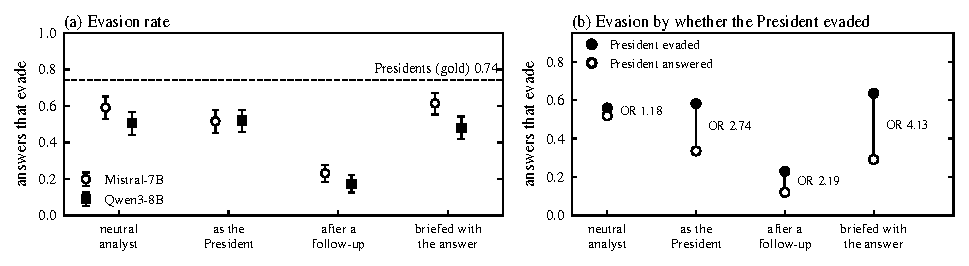
\includegraphics[width=\textwidth]{figures/fig_e25_audit.pdf}
\caption{E25b, labelled by the frozen instrument. (a)~Share of LLM answers that evade, with 95\% cluster-bootstrap intervals (dashed line: the Presidents' gold rate). (b)~The association as plain rates: the share of answers that evade where the President evaded (filled) and where the President answered (open), pooled over the two models, with the odds ratio beside each pair.}
\label{fig:audit}
\end{figure*}}

\newcommand{\FigureSwap}{%
\begin{figure*}[t]
\centering
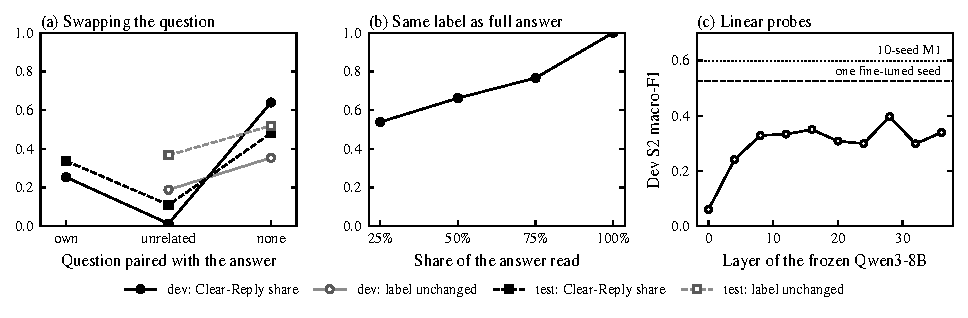
\includegraphics[width=\textwidth]{figures/fig_e25_swap_probe.pdf}
\caption{E25a, c and d. (a)~Each answer paired with its own question, a question from another interview, or none. ``Label unchanged'' is the share of items keeping their own-question label. (b)~Agreement of the label on the first 25/50/75\% of the answer with the full-answer label (dev). (c)~Linear probes on every fourth layer of the frozen Qwen3-8B-Base.}
\label{fig:swap}
\end{figure*}}

\newcommand{\FigureStageOne}{%
\begin{figure*}[t]
\centering
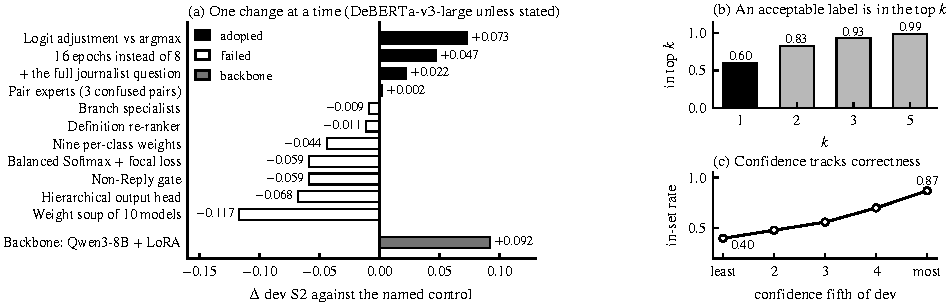
\includegraphics[width=\textwidth]{figures/fig_stage1.pdf}
\caption{Stage~1 on dev \Stwo{}. (a)~Each change against its named control (E0--E13): per model for training and input changes, per system for the rest. (b, c)~The Qwen3-8B classifier ranks better than it decides, and correctness rises with confidence (3 epochs, seeds 0--2).}
\label{fig:stage1}
\end{figure*}}

\newcommand{\FigureFrontier}{%
\begin{figure}[t]
\centering
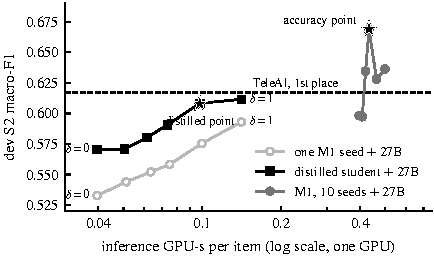
\includegraphics[width=\columnwidth]{figures/fig_frontier.pdf}
\caption{The cascade on dev: \Stwo{} against inference GPU-s per item, for deferral rates $\delta = 0, 0.1, 0.2, 0.3, 0.5, 1$ (left to right on each curve, first scoring, one option order). All times are on one GPU (Appendix~\ref{sec:impl}). TeleAI's GPU time is not published.}
\label{fig:frontier}
\end{figure}}

\newcommand{\FigureStageThree}{%
\begin{figure*}[t]
\centering
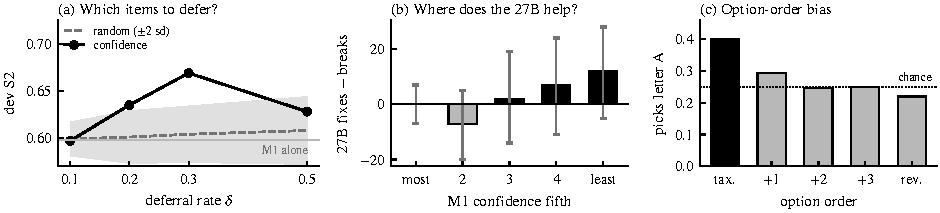
\includegraphics[width=\textwidth]{figures/fig_stage3.pdf}
\caption{Stage~3 (E19--E22), registered tests of the Stage~2 result. (a)~Confidence routing against 200 random routings. (b)~Net fixes of the 27B by M1's confidence, on 1,067 leak-free training rows. (c)~How often the 27B picks the first option, by order.}
\label{fig:stage3}
\end{figure*}}

\newcommand{\FigureRelation}{%
\begin{figure}[t]
\centering
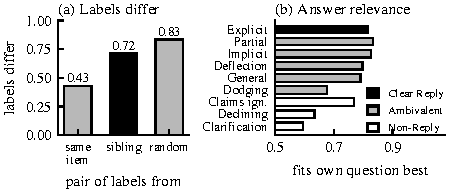
\includegraphics[width=\columnwidth]{figures/fig_relation.pdf}
\caption{Evasion is a relation (E24). (a)~Share of dev label pairs from two annotators that differ: same item, two sub-questions of one answer, random items. (b)~Share of three random questions under which the answer is less likely than under its own, by gold label (train): Partial, Implicit, Deflection and General answers are as relevant as Explicit ones.}
\label{fig:relation}
\end{figure}}

\newcommand{\FigurePrecision}{%
\begin{figure}[t]
\centering
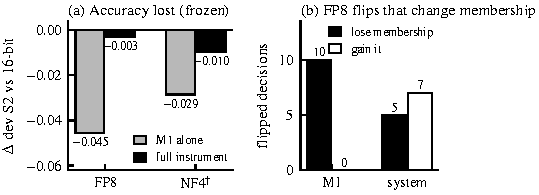
\includegraphics[width=\columnwidth]{figures/fig_precision.pdf}
\caption{E26 on dev, each format against 16-bit on the same GPU type. (a)~\Stwo{} lost, both with frozen parameters. (b)~FP8 flips that change reference-set membership. $^{\dagger}$Lower bound: 27B records missing for 60 NF4 items.}
\label{fig:precision}
\end{figure}}


\title{Evasion Is a Relation: A Confidence-Routed Cascade for\\Political Question Evasion, and What It Measures}

\author{%
  \begin{tabular}[t]{@{}c@{\hspace{1.1em}}c@{\hspace{1.1em}}c@{\hspace{1.1em}}c@{}}
    Vidvathama R & Siddarth Gottumukkula & Sanjana Reddy Vonteri & Shashikanta Sahoo \\
    {\normalfont\small 2024122002} & {\normalfont\small 2023102040} &
    {\normalfont\small 2026901007} & {\normalfont\small 2026900007}
  \end{tabular}
  \AND
  {\normalfont Team Nier\_ANLP} \\
  {\normalfont International Institute of Information Technology, Hyderabad}}

\hypersetup{pdftitle={Evasion Is a Relation: A Confidence-Routed Cascade for Political Question Evasion, and What It Measures},
  pdfauthor={Vidvathama R, Siddarth Gottumukkula, Sanjana Reddy Vonteri, Shashikanta Sahoo (Team Nier\_ANLP, IIIT Hyderabad)}}

\begin{document}
\maketitle
\begin{abstract}
SemEval-2026 Task~6 (CLARITY) asks how a politician's answer responds to one interview question, as one of nine evasion types (Subtask~2) or three clarity levels (Subtask~1).
We ask five questions in turn, each registered before its experiments and each raised by the answer to the one before.
A controlled encoder study finds that architectural changes do not help, while swapping only the backbone for a LoRA-tuned Qwen3-8B does (+0.092 Subtask-2 macro-F1 per model, on ten of ten paired seeds).
That classifier ranks better than it decides, so a 27B LLM chooses among its top four labels for the 30\% of items it is least sure of.
The resulting cascade scores 0.650 (Subtask~2) and 0.788 (Subtask~1) on the development set with 1.4 LLM calls and about 1.6k LLM input tokens per item, against 0.617 and 0.812 at 1.94 calls and about 7.3k tokens for the winning system.
A distilled single-model variant matches the ten-model classifier at a quarter of its GPU time.
We then freeze the cascade and use it as an instrument.
The labels of one answer change with its sub-question far more often than annotator noise explains, and pairing an answer with an unrelated question cuts the Clear-Reply share from 25\% to 1\%, so evasion is a relation between a question and an answer.
Put to two open LLMs, a neutral analyst's evasions show no clear link to the Presidents' (odds ratio 1.18), but in the President's role the models answer directly the questions the Presidents answered directly (2.74, exploratory), and a follow-up turns 66\% of their evasions into replies.
Finally, running the classifier in FP8 costs it 0.045 Subtask-2 macro-F1 with all parameters frozen, while the full cascade loses 0.003.

\end{abstract}

\section{Introduction}
\label{sec:intro}
\FigurePath

Politicians often answer the question they would have liked to be asked.
\citet{thomas-etal-2024-never} turned this observation into a two-level taxonomy of response clarity and evasion, and SemEval-2026 Task~6 \citep{thomas-etal-2026-semeval} made it a shared task.
The task was won by pipelines that call a large language model (LLM) several times per item \citep{shi-etal-2026-teleai}, while fine-tuned encoders levelled off near 0.50 macro-F1 on the nine-way subtask.
A leaderboard shows which system is best, but not why the others stop where they do, nor what a good classifier of evasion could be used to find out.

This paper addresses those two questions in five stages (Figure~\ref{fig:path}). Figure~\ref{fig:system} shows the system it builds and how it is used.
At each stage we wrote down a hypothesis, a prediction and a decision rule before running anything, and the result of each stage set the question of the next.

\noindent Our contributions follow the same order. First, controlled evidence that a stronger pretrained backbone helps where structural changes do not. Second, a cascade at 0.650 Subtask-2 macro-F1 with 1.4 LLM calls per item, and a distilled variant at a quarter of the classifier's GPU time. Third, evidence that evasion is relational, and an exploratory LLM audit in which, in the President's role, models answer directly what the Presidents answered directly. Fourth, a measurement of what reduced precision costs the cascade.
Every system comparison is on the 308-item development set, since the test labels were never released.
Many registered hypotheses failed. We report them where they fell, because each failure changed what we did next.

\section{Task, Data and Protocol}
\label{sec:task}
\FigureSystem

\paragraph{Task.}
Each item is a triple $x = (q, Q, a)$ from a U.S.\ presidential interview \citep{thomas-etal-2024-never}: a sub-question $q$ (median 15 tokens), the journalist's full turn $Q$ it was split from (62 tokens) and the President's whole answer $a$ (266 tokens).
Subtask~2 (\Stwo{}) asks for one of nine evasion types $\mathcal{Y}_9$, describing how $a$ responds to \emph{that} sub-question, and each type fixes one of three clarity levels for Subtask~1 (\Sone{}, Table~\ref{tab:taxonomy}).
Like the top systems, we predict the nine-way type and map it to the clarity level.

\begin{table}[t]
\centering
\small
\setlength{\tabcolsep}{3.5pt}
\begin{tabular}{@{}llrr@{}}
\toprule
Evasion type (\Stwo{}) & Clarity level (\Sone{}) & Train \% & Dev sets \\
\midrule
Explicit            & Clear Reply     & 30.5 & 115 \\
\midrule
Implicit            & Ambivalent      & 14.2 & 99 \\
Dodging             & Ambivalent      & 20.5 & 96 \\
General             & Ambivalent      & 11.2 & 113 \\
Deflection          & Ambivalent      & 11.0 & 51 \\
Partial/half-answer & Ambivalent      & 2.3  & 14 \\
\midrule
Declining to answer & Clear Non-Reply & 4.2  & 17 \\
Claims ignorance    & Clear Non-Reply & 3.5  & 15 \\
Clarification       & Clear Non-Reply & 2.7  & 4 \\
\bottomrule
\end{tabular}
\caption{The taxonomy. Train \% is the share of the 3,448 training labels. Dev sets is the number of the 308 dev items whose reference set contains the type.}
\label{tab:taxonomy}
\end{table}

\paragraph{Data.}
Train has 3,448 items with one label each.
Dev has 308 items with three annotators: 125 are unanimous, 150 split two to one and 33 receive three labels, so the reference set $G_i$ of an item holds one to three types.
The 237 test items have two annotators, but their labels were never released, so every comparison is on dev, and we also rescore dev against each of its three two-annotator subsets (the test regime).
One property shapes the whole paper: 69\% of training rows share their answer with another sub-question of the same turn (\emph{siblings}).

\paragraph{Metric.}
\Stwo{} is scored by multi-reference macro-F1: a prediction is a true positive if it lies in $G_i$, and every class counts equally.
It rewards both the \emph{in-set rate} and \emph{coverage} of rare classes.
Always predicting Explicit scores 0.060, TF-IDF with logistic regression 0.257, and a human annotator against the other two 0.684.

\paragraph{Protocol.}
Epochs, calibration and routing thresholds are chosen on the \emph{train slice}, a fixed stratified 10\% of train (345 rows).
The few parameters that must be fitted on dev are chosen by 5-fold nested cross-validation, and we report the first split and the mean over ten splits.
A \emph{system} averages seeds and applies logit adjustment \citep{menon2021longtail}, $\hat y = \arg\max_c \bar p(c \mid x)/\pi_c^{\tau}$ with $\pi_c$ the train prior and $\tau$ the only fitted parameter.
Claims rest on ten paired seeds, and a change must first pass a three-seed screen (+0.015, at least two of three seeds up).
Before each experiment we registered its hypotheses, predictions and decision rules. Later changes were logged as amendments before results were seen.
From \S\ref{sec:measure} on, every label comes from one \emph{frozen} system, so no parameter changes between experiments.

\section{Related Work}
\label{sec:related}

\paragraph{The task and its systems.}
\citet{thomas-etal-2024-never} introduced the clarity and evasion taxonomy and found that predicting the nine-way type and mapping it up beats predicting clarity directly.
In the shared task \citep{thomas-etal-2026-semeval}, fine-tuned encoders levelled off near 0.50 on test \Stwo{} and the strongest systems prompted LLMs.
TeleAI \citep{shi-etal-2026-teleai} won with three confidence-routed chain-of-thought stages on DeepSeek-V3 (1.94 calls per item, dev 0.617 \Stwo{} and 0.812 \Sone{}), and also reported a fine-tuned Qwen2.5-7B at 0.495.
ChulaNLP \citep{peerachaidecho-rutherford-2026-chulanlp} passed a DeBERTa model's top five labels to a prompted LLM (dev 0.52).
The parts of our cascade are not new. We add a controlled account of which parts matter, and its use as an instrument.

\paragraph{Cascades and LLM choosers.}
Sending only some inputs to a larger model, as FrugalGPT \citep{chen2023frugalgpt} does for LLM APIs, is the idea behind our router.
LLMs choosing among lettered options are sensitive to option order \citep{zheng2024large}, which we measure and correct, and we distil the adjudicator into the classifier with soft targets \citep{hinton2015distilling}.

\paragraph{Evasion as a property of the exchange.}
Conversation analysis defines evasion relative to the question: an answer evades by failing to meet the agenda the question sets \citep{clayman-2001-answers}.
\citet{alvarez-morrier-2025-measuring} score answer quality by how identifiable an answer is among others given its question. We test whether such relevance captures the taxonomy's labels, and we use LLMs as speakers with no political stake under the same instrument.

\section{Stage 1: What Limits a Fine-Tuned Classifier?}
\label{sec:classifier}
\FigureStageOne

\step{Question.}
Label noise, a decision rule that does not fit the metric, missing knowledge and labels too subtle for 3,448 examples each predict a different fix.
We tested these explanations on DeBERTa-v3-large \citep{he2023debertav3}, fully fine-tuned with a nine-way head, changing one thing at a time against a named control (Figure~\ref{fig:stage1}a).

\step{Result: structure fails, the decision rule and training length help.}
Every system averages the softmax outputs of ten seeds that differ only in their random seed, which reduces variance, and then applies a one-parameter logit adjustment, $\hat y = \arg\max_c \bar p(c \mid x)/\pi_c^{\tau}$.
Dividing by the train prior $\pi_c$ lifts the rare classes that an argmax under-predicts and that macro-F1 weights equally. It raised an encoder system from 0.365 to 0.438 (E4), whereas nine free class weights reached only 0.394 and overfit dev (in-fold gain +0.098).
A one-parameter logit adjustment, longer training and the full journalist question improved the model: 0.315 to 0.384 per model, 9 of 10 seeds up.
Every structural idea failed: hierarchies did not beat a flat softmax that already scores all nine labels jointly, rebalanced losses over-corrected towards rare classes (Explicit F1 0.68 $\rightarrow$ 0.32), and boundary experts rarely overturned decisions the flat model made from the same input.
The definition re-ranker is the telling failure: gold was in the encoder's top three for 90\% of items, yet a second encoder given label definitions chose worse.

\step{Why: the model, not the labels.}
Of the encoder ensemble's predictions, 44.5\% fell outside the reference set, 53 of them on items where all three annotators agreed, while a human annotator scores 0.684 against the other two.
So label noise does not explain the gap, and nothing trained on the same 3,448 rows moved the system.

\step{Hypothesis E13: the gap is knowledge.}
We replaced only the backbone with Qwen3-8B-Base \citep{qwen3}, adapted with LoRA \citep{hu2022lora} (rank 16, all linear layers) and a new linear head on the last token, keeping the data, input, loss and selection rule.
We expected the gain to concentrate on the commitment boundary (Explicit--Implicit--General), where the encoder's errors sit, and on unanimous items.
The gain was +0.092 \Stwo{} and +0.095 \Sone{} per model on all ten seeds, more than the whole encoder track gained. The 10-seed system reached 0.543 \Stwo{} and 0.746 \Sone{} (95\% CI of the gain over DeBERTa \ci{+0.054}{+0.224}).
The location was not as expected: the gain was broad (seven of nine classes), largest on Claims ignorance (+0.40) and Declining (+0.22), the classes that depend on recognising \emph{what kind of statement} an answer is.
Twelve epochs, adopted on the slice (+0.084 F1, 3/3 seeds), became the default.

\step{What it raised.}
The 8B classifier ranks far better than it decides, and it knows when it is unsure (Figure~\ref{fig:stage1}b--c).
Most remaining errors are choices among a few candidates it already ranks highly, made where it is unsure.

\section{Stage 2: Can a Larger Model Choose Among the Candidates?}
\label{sec:cascade}
\FigureFrontier

\step{M1, the candidate generator (E14).}
On ten seeds the 12-epoch classifier scores \pmsd{0.525}{0.042} per model (+0.049 over 3 epochs, 8/10 up) and 0.598 \Stwo{} / 0.743 \Sone{} as a system (M1, Figure~\ref{fig:system}).
Three registered checks shaped the next module.
An oracle re-deciding the 30\% least confident items within the top three would reach 0.727, but a \emph{random} choice there lowers \Stwo{} to 0.587: M1's first choice carries information, so an adjudicator must be \emph{fused} with M1, not substituted for it.
Candidate sets defined by probability mass did not transfer from the slice to cross-fitted rows (coverage 0.98 vs 0.76) while rank-based sets did, so $C(x)$ is the top four.
And five seeds did not score within 0.01 of ten as predicted (0.555 vs 0.598), so M1 kept ten seeds and became the dominant cost.

\step{M3, the adjudicator (E15).}
Qwen3.8-27B-FP8, run locally without thinking, reads the label definitions, a guide to the most-confused pairs and the item, and answers with one letter among the four candidates, and $q(c \mid x)$ is the softmax over the letters' log-probabilities.
On deferred items the label is $\arg\max_{c \in C(x)} \lambda \log \bar p + (1-\lambda) \log q - \tau \log \pi_c$, with $(\lambda, \tau)$ fitted by nested CV. Other items keep M1's answer.
A screen on 300 cross-fitted training rows refuted two registered design assumptions: retrieved examples \emph{hurt} (fused accuracy 0.353 with none, 0.330 with ten), and a 304B mixture-of-experts model was worse than the local 27B (0.317).

\step{Result, and a correction.}
The first dev analysis showed no gain. Explaining it, we found a bug that shared one $\tau$ between deferred and kept items and so switched off M1's logit adjustment on the 64\% of items meant to keep M1's answer.
Corrected, deferring 30\% of items gives 0.669 \Stwo{} (0.660 over ten splits) and 0.798 \Sone{}, +0.067 \ci{+0.009}{+0.124} over M1 with the fitted parameters held fixed (Figure~\ref{fig:frontier}), with 33 items moving into the reference set and 9 out (McNemar $p = 0.0003$).
Deferring \emph{every} item is worse (0.609 over ten splits): where M1 is confident, the LLM is the weaker reader.

\step{Where the cost goes (E16).}
Timed on one GPU, an M1 seed costs 0.040 GPU-s per item and a 27B call 0.101, so the ten seeds are 92\% of the cascade's inference time and the 27B only 8\%.
Removing prompt parts lowered dev \Stwo{} in the expected order, each step within noise (full 0.660, no confusion guide 0.637, no definitions 0.628, neither 0.617), so the full prompt stayed.
With $K \le 5$ seeds M3 adds only +0.021 to +0.031 at $\delta = 0.3$, against +0.071 at $K = 10$.

\step{M4, distillation for cost (E17--E18).}
M3 relabelled every training row over its cross-fitted top four, and one student learned from $\tfrac12$gold $+ \tfrac12 q$, a weight fixed in advance \citep{hinton2015distilling}.
The student beats M1 per model (0.573 vs 0.525, 9/10 seeds up) and is far better calibrated (mean top probability 0.58 vs 0.84), yet it ranks its errors no better (AUROC 0.686 for both), against our prediction.
With M3 it missed the registered target at $\delta = 0.3$ (0.591 vs 0.614). At $\delta = 0.5$ it reaches 0.608 \Stwo{} / 0.790 \Sone{} at 0.098 GPU-s per item, above the ten-seed M1 alone at a quarter of its time, and it beats 25 of the 30 undistilled (seeds, $\delta$) points with less GPU time.
Ensembles of students add almost nothing (+0.005 from one to ten, vs +0.065 for M1 seeds): students trained towards the same targets lose the diversity seed ensembles feed on.
We froze an \emph{accuracy} point (M1 $\times$ 10 + M3, $\delta = 0.3$) and a \emph{distilled} point (one student + M3, $\delta = 0.5$).

\step{What it raised.}
The accuracy point rested on one ensemble whose M3 gain was twice that of any smaller one, on parameters fitted on 308 items, and, for the distilled point, on a $\delta$ chosen after the registered one failed.

\section{Stage 3: Which Gains Survive?}
\label{sec:robust}
\FigureStageThree

\step{Question.}
The Stage~2 gain rests on one ensemble, one adjudicator and one prompt. Each simpler alternative predicts a specific failure, so we registered one test per alternative (Figure~\ref{fig:stage3}), decided on training rows or held-out folds, never on dev.

\step{Result.}
Three findings change how the cascade should be read.
On 3,448 cross-fitted training rows the cascade gains a small but significant +0.014 \ci{+0.002}{+0.026}, less than on dev, where its parameters were fitted.
The gain is carried by the two parts a simpler system lacks: confidence routing, which no random routing matches (Figure~\ref{fig:stage3}a), and fusion (the 27B alone over all nine labels scores 0.591, below M1's 0.598, and deciding the deferred items alone scores 0.631).
The 27B breaks as many confident decisions as it fixes and helps only where M1 is unsure (b), which is why a learned fix/break router lost to confidence at all four budgets.
And the 27B's decisions depend on more than the item.
LLMs choosing among lettered options are known to prefer some positions over others \citep{zheng2024large}, and the 27B prioritises option A: in taxonomy order it picks A for 40\% of items, against 22--29\% in the other orders and 25\% by chance (Figure~\ref{fig:stage3}c). Because slot A usually holds Explicit in taxonomy order, a preference for A is also a preference for Explicit. Two orders of the same four candidates give the same pick on only 72\% of dev items, so we average four, which costs four calls and moved the system by +0.011 at split 0 but +0.002 over ten splits.
Two results also changed what we claim. A student taught by M1's own soft targets came within the registered margin of the M3-taught one, so the distilled point is a soft-target effect, not ``the LLM's knowledge''. Transcript artifacts in 97\% of test answers changed 15.6\% of M1's labels when injected into dev, so test predictions use normalised text.

\step{The frozen instrument (E23).}
Re-scoring every record on one serving setup of the 27B with order-averaged $q$ gives the final operating points (Table~\ref{tab:final}), slightly lower than the Stage~2 scores because all 27B decisions now come from one scoring run.
Averaging four orders costs four 27B calls per deferred item, so the accuracy point, 0.650 \Stwo{} (0.639 over ten splits) and 0.788 \Sone{}, makes 1.43 calls per item and takes 1.36$\times$ M1's GPU time (Table~\ref{tab:final} gives the one-order variants).
Against the winning system it is higher on \Stwo{} and lower on \Sone{}, with three quarters of its calls and a fifth of its LLM input tokens (its GPU time is not published).
Every setting of the accuracy point is fixed in one file (Appendix~\ref{sec:impl}). From here on it is the \emph{instrument}, and nothing in it is refitted.

\begin{table}[t]
\centering
\small
\setlength{\tabcolsep}{2.2pt}
\begin{tabular}{@{}lcccc@{}}
\toprule
System (dev) & \Stwo{} & \Sone{} & calls & GPU-s \\
\midrule
DeBERTa-v3-large, 10 seeds & 0.405 & 0.648 & 0 & -- \\
M1: Qwen3-8B, 10 seeds & 0.598 & 0.743 & 0 & 0.397 \\
\textbf{Accuracy point} (M1 + M3) & \textbf{0.650} & \textbf{0.788} & 1.43 & 0.538 \\
\quad one option order & 0.639 & 0.787 & 0.36 & 0.433 \\
\textbf{Distilled point} (student + M3) & \textbf{0.608} & \textbf{0.785} & 2.30 & 0.266 \\
\quad one option order & 0.599 & 0.784 & 0.57 & 0.098 \\
\midrule
TeleAI, 1st place & 0.617 & 0.812 & 1.94 & n/a \\
Human vs.\ two others (2-ann.) & 0.684 & -- & -- & -- \\
\bottomrule
\end{tabular}
\caption{Final systems (E23, one serving setup, nested-CV split 0). Calls: 27B calls per item (four per deferred item with order-averaged $q$). GPU-s: inference per item on one GPU (Appendix~\ref{sec:impl}). TeleAI uses ${\sim}$7.3k LLM input tokens per item, the accuracy point ${\sim}$1.6k.}
\label{tab:final}
\end{table}

\step{What it raised.}
The cascade's gain is now explained, but not what its labels mean: question--answer relevance, tried as a router feature (E22), barely predicted its errors ($\rho = +0.095$).
If the label is not a property of the answer's relevance, what is it a property of?

\section{Stage 4: What Does the Instrument Measure?}
\label{sec:measure}

\subsection{Labels across the sub-questions of one answer (E24)}
\label{sec:relation}
\FigureRelation

\step{Question.}
If evasion were a property of an answer's style, one answer would get one label whatever it was asked. Answers shared by several sub-questions test this (CPU only, existing outputs).

\step{Result.}
Of the 3,079 training pairs of siblings (two sub-questions, one answer), 61.5\% carry different evasion types and 40.6\% different clarity levels.
This is not annotator noise: on dev, moving to a sibling's sub-question changes the label almost as often as moving to an unrelated exchange, and far more often than two annotators disagree on the same item (Figure~\ref{fig:relation}a).
The label belongs to the pair, not to the answer.
M1 already behaves accordingly, repeating its label on only 19\% of the 58 dev sibling pairs with disjoint annotator sets.

\step{Relevance is not answerhood.}
Political scientists score answer quality by how specific an answer is to its question \citep{alvarez-morrier-2025-measuring}. We computed this with the frozen Qwen3-8B as the gain in the answer's log-likelihood under its own sub-question over three random ones.
It is ordered across the nine labels (Kruskal--Wallis $p = 2 \times 10^{-12}$) but barely discriminative (AUROC 0.566 for Clear Reply against the rest): Partial, Implicit, Deflection and General answers fit their own question as well as Explicit ones do (Figure~\ref{fig:relation}b).
An answer can be \emph{about} the question without \emph{answering} it, which is the distinction the taxonomy draws.
Five further module ideas (epistemic-uncertainty routing, joint decoding of siblings, a parameter-free metric-optimal decision rule, single-order debiasing, conformal candidate sets) were tested on existing outputs and rejected before any new run (Appendix~\ref{sec:ledger}).

\subsection{Does the instrument read the question causally? (E25a)}

\step{Registered prediction (H25a-1).}
An answer paired with a question from another interview has, by the taxonomy's definition, not replied to it.
If the instrument models the relation, the Clear-Reply share should fall by at least half and at most 50\% of items should keep their label. If it labels answer style, labels should persist.
This is not obvious: training never showed a mismatched pair.

\step{Result.}
Held (Figure~\ref{fig:swap} in the appendix, left).
With an unrelated question the Clear-Reply share falls from 0.253 to 0.013, only 18.8\% of items keep their label, and 62 of the 78 Clear Replies become Dodging. The label-free replication on test runs in the same direction (0.338 to 0.110).
Without any question the share \emph{rises} to 0.640: with nothing asked, nothing can be evaded.
The instrument models the relation, the precondition for using it on new speakers.

\subsection{Does the question or the speaker drive evasion? (E25b)}

\step{Design.}
If evasion is relational, it could be driven by the question (some questions are hard to answer for anyone) or by the speaker (Presidents evade strategically).
We put the 308 dev sub-questions (191 interview turns) to two open instruction-tuned LLMs, Mistral-7B-Instruct-v0.3 \citep{jiang2023mistral} and Qwen3-8B with thinking off \citep{qwen3}, in four conditions that each differ from P in one factor. \textbf{N} is a neutral analyst with no stake, \textbf{P} the President in that interview on its date, \textbf{F} P followed by ``With respect, you haven't answered the question'', and \textbf{B} P with the President's real answer as private notes.
The frozen instrument labelled all 2,464 answers against their sub-questions. Statistics use a cluster bootstrap over turns and Mantel--Haenszel odds ratios pooled over models.

\FigureAudit

\begin{table}[t]
\centering
\small
\setlength{\tabcolsep}{3pt}
\begin{tabular}{@{}llll@{}}
\toprule
 & Registered prediction & Result & Verdict \\
\midrule
a-1 & unrelated question: CR $\le \tfrac12$ & 0.253 $\rightarrow$ 0.013 & held \\
b-1 & no stake: OR $\ge 1.5$ & 1.18 & failed \\
b-2 & stake: P $-$ N $\ge +0.10$ & $-$0.031 & failed \\
b-3 & pursuit: $\ge$50\% replies & 66\% & held \\
b-4 & notes: indirect $-$ non $\ge +0.15$ & +0.113 & failed \\
c & half answer: $\ge$70\% agree & 66\% & failed \\
d-1 & frozen probe: \Stwo{} $\ge 0.45$ & 0.397 & failed \\
d-2 & probe: siblings same $\ge$30\% & 45\% & held \\
\bottomrule
\end{tabular}
\caption{E25's registered hypotheses (dev, frozen instrument). CR is the Clear-Reply share and OR the odds ratio, shown beside each pair in Figure~\ref{fig:audit}b.}
\label{tab:e25}
\end{table}

\step{Results.}
Both registered hypotheses about the question and the stake failed (Table~\ref{tab:e25}, Figure~\ref{fig:audit}): a neutral analyst does not evade more on the questions the Presidents evaded (OR 1.18), and playing the President does not raise the evasion \emph{rate} ($-$0.031).
In the President's role, though, the same models evade on the questions the Presidents evaded (OR 2.74 \ci{1.87}{4.17}, with 3.0 for Mistral and 2.5 for Qwen). We did not register this comparison, so it is exploratory.
In plain rates (Figure~\ref{fig:audit}b), the neutral analyst evades on 56\% of the questions the Presidents evaded and on 52\% of those they answered. In the President's role the models evade on 58\% and 34\%.
The move therefore comes from the questions the Presidents answered directly, which the models now also answer directly, not from the questions the Presidents dodged. A neutral analyst addressed as ``Mr.\ President'' evades about half of everything, because it is not the addressee.
The role changes \emph{where} models evade, not how often (52\% against 55\%). A question's answerability shows only for a speaker who can answer it, and our data cannot tell this apart from strategic evasion.
Labelling N and P with one instrument removes a question prior that acts alike on every answer, not one that interacts with answer style, and the question-only control was degenerate.
Pursuit works: a follow-up turns 66\% of evasive answers into clear replies.
With the President's answer as notes, indirect answers become replies more often than non-answers, by less than the registered margin. Condition effects survive a length covariate, but the role odds ratio was not length-adjusted.

\step{Is the instrument valid on LLM text?}
The registered human check was dropped for lack of time. Without labels, the instrument is \emph{more} confident on LLM answers than on the Presidents' (seed agreement 0.81 vs 0.73), though confident errors remain possible.

\subsection{Is there a shortcut? (E25c--d)}
A shortcut would exist if evasion were visible early in an answer or encoded in the frozen base model. Neither holds (Figure~\ref{fig:swap}b--c).
Half an answer agrees with the full-answer label on only 66\% of items: refusals show early, General and Dodging only at the end.
Linear probes on the frozen Qwen3-8B-Base reach 0.397 \Stwo{} at best, against 0.525 for one fine-tuned seed, and they give disjoint siblings the same label 45\% of the time, against 19\% for M1. Fine-tuning is what ties the label to the question.

\step{What it raised.}
Measuring evasion needs the whole answer and the fine-tuned ten-seed ensemble, so one lever that leaves the instrument's model, and so its labels, unchanged is numeric precision.

\section{Stage 5: Can the Instrument Be Made Cheaper?}
\label{sec:precision}
\FigurePrecision

\step{Design and predictions.}
The ten seeds are three quarters of the instrument's GPU time.
Unlike distillation (\S\ref{sec:cascade}), reduced precision changes only the arithmetic, so we ran the frozen M1 at reduced precision and compared each format with 16-bit on the same GPU type.
FP8 (8-bit weights and activations) was compared through the full instrument, NF4 (4-bit weights, as in QLoRA, \citealp{dettmers2023qlora}) at the level of M1.
We predicted that FP8 would keep $\ge$98\% label agreement and \Stwo{} within 0.01 (H26-1) and be at least 1.3$\times$ faster at the same batch size (H26-2).
The non-obvious prediction, H26-4, was that FP8's flips would fall where the 27B re-decides, so the instrument would lose less than M1.

\step{Result.}
Both FP8 predictions about M1 failed (Figure~\ref{fig:precision}c): FP8 changes 3.9\% of the ensemble's argmax labels (17 of M1's final decisions) and lowers M1's \Stwo{} by 0.045 with the parameters frozen.
We ran FP8 on the native FP8 tensor cores of an RTX PRO 6000 (Blackwell). As implemented it still lowers batched throughput to 0.83$\times$, because activations are quantized in unfused operations around each FP8 matrix product. Reported FP8 speed-ups rely on kernels that fuse these steps into the matrix product, which we did not use. FP8 also barely changes peak memory (0.96$\times$), since the embeddings, norms and head stay in 16 bit.
Applied to the accuracy point's one-GPU cost, the slower M1 would raise it from 0.538 to 0.619\,\mbox{GPU-s} per item (+15\%).
H26-4 held on its two registered counts (Figure~\ref{fig:precision}a,b): 71\% of FP8's 17 flips land on items the 27B re-decides, twice the chance rate, and the system flips 16 decisions against M1's 17.
All 10 of M1's membership-changing flips lose reference-set membership, whereas the system's go both ways (5 lose, 7 gain), so with the same frozen parameters it loses 0.003 against M1's 0.045.
The cascade does not undo the flips but turns a one-sided loss into noise.
NF4 changes more (86.7\% ensemble agreement) and meets our registered QLoRA trigger.
It saves memory but not time: peak memory falls to 0.67$\times$ (16.8 to 11.3\,GB), short of the 0.4$\times$ we predicted, while batch-1 latency rises from 169 to 259\,ms, because the 4-bit weights are stored compactly but computed in bf16.
Its throughput (0.82$\times$) is not like for like, since the 16-bit reference ran split over two cards.
Its cascade comparison is incomplete (27B records are missing for 60 of 136 deferred items), so we draw no conclusion from it.
Precision is not a cost lever with these kernels.

\section{Conclusion}
\label{sec:conclusion}

A classifier on this task is limited by knowledge, not structure, and ranks better than it decides. A 27B adjudicator consulted only where it is unsure lifts dev \Stwo{} to 0.650 with fewer LLM calls and tokens than the winning system.
As a frozen instrument, it shows that evasion is a relation between question and answer, and that in the President's role LLMs answer directly what the Presidents answered directly (exploratory), which motivates a question-side prior as the next module. Run in FP8 without fused kernels, the classifier loses 0.045 \Stwo{} and is not faster, while the cascade loses 0.003.


% Not counted in the page limit: Limitations, challenges and future work, just before the references.
% Course rule: this section holds only challenges, limitations and future work (no results), and sits just
% before the references; it is not counted in the page limit. Each limitation names the step that addresses it.
\section*{Limitations, Challenges and Future Work}

\paragraph{One small development set.}
Every number is on 308 dev items, because the test labels were never released and the evaluation server has closed.
Differences between systems therefore carry wide intervals, and parameters fitted on dev (by nested cross-validation) use dev labels.
\emph{Next step:} score the frozen test predictions in the repository as soon as the organisers release the test labels, and re-run the instrument, unchanged, on a second evasion corpus such as parliamentary question periods.

\paragraph{Validity of the instrument on LLM text.}
The instrument was trained on presidential speech; our check on LLM answers is label-free, so it cannot rule out confident errors.
\emph{Challenge:} the registered human annotation of LLM answers was dropped for lack of time.
\emph{Next step:} have two annotators label a stratified sample at the clarity level, blind to model and condition, and use the instrument only if its agreement with them is within 0.10 of their agreement with each other, as registered.

\paragraph{Breadth of the LLM audit.}
The audit covers two model families, one of which shares a family with the 27B judge. The role effect was not a registered hypothesis.
\emph{Challenge:} two further families (Llama-3.1, OLMo-2) failed to load on the shared GPU because of context-length and memory settings.
\emph{Next step:} re-run them with their own GPU and context limits, adjust the role odds ratio for answer length, and register the role effect as a hypothesis for that replication.
Role play is also not politics: an LLM has no career at stake, so ``role'' here means the prompt, and conclusions about real politicians would need human studies.

\paragraph{Reproducibility of LLM decisions.}
The adjudicator's decisions depend on the serving stack, the GPU and the option order, not only on the weights and the item, and we never repeated a run, so its own run-to-run noise is unmeasured.
\emph{Next step:} repeat the 27B's dev run several times, pin the serving software and hardware in the frozen file, and report decision agreement across repeats alongside every result that uses an LLM.

\paragraph{Cost measurements.}
GPU time was measured with batched inference over the 308 dev items on one GPU type. Per-item cost depends on batch size and hardware, and our reduced-precision runs used unfused FP8 kernels, so they measure accuracy under quantization but not the speed a production kernel would give.
The winning system's cost is known only in calls and tokens.
\emph{Next step:} serve M1 through fused FP8 kernels, retrain the adapter on the 4-bit base (QLoRA), as our registered trigger requires, score the 27B on every item NF4 defers so its cascade comparison is complete, and report latency at batch size one alongside throughput.

\paragraph{Labels and classes.}
Training items carry one annotator's label, so the models cannot learn how disputed an item is, and the any-annotator metric credits labels that most annotators rejected.
Partial/half-answer and General remain the weakest classes.
\emph{Next step:} train on soft labels where several annotations exist, and add targeted contrast examples for the weakest classes.
We also cannot rule out that the pretraining data of the LLMs include the public interview transcripts.

\paragraph{Process challenges.}
Shared hardware forced two deviations from our plans (a different GPU type for E25, and two LLM families dropped), both logged before results were seen.
A fusion bug in our own analysis was found and corrected in the log. Every analysis now reproduces its saved predictions before it reports a number.

\section*{Ethical Considerations}

The instrument labels the form of an answer relative to a question, not its truth or the speaker's intent, and its output should not be read as a verdict on any politician.
The LLM ``Presidents'' of Section~\ref{sec:measure} are role-play prompts, not models of real people's views.
All data are the public interview transcripts released for the shared task.


\bibliography{references}

\clearpage
\appendix
% Appendix (at most two pages): the experiment ledger, implementation details and the frozen instrument.
% Sources: docs/experiment_log.md (E0-E26), docs/raw/*, code/experiments/e25/frozen_system.json.
\section{Experiment Ledger}
\label{sec:ledger}

Table~\ref{tab:ledger} lists every experiment in the order it ran. The hypotheses, decision rules and amendments are in the repository's pre-registered log.

\begin{table*}[t]
\centering
\scriptsize
\setlength{\tabcolsep}{4pt}
\begin{tabular}{@{}lllll@{}}
\toprule
Exp. & Question & Key result (dev \Stwo{}) & Verdict & Led to \\
\midrule
E0--E3 & Where does DeBERTa fail? & gold in top 3: 90\% & -- & decision rules \\
E4 & Decision rule? & LA 0.365 $\rightarrow$ 0.438 & held & LA in every system \\
E5, E6 & Taxonomy routing, definition re-ranker? & 0.369, 0.354 vs 0.365 & failed & knowledge, not structure \\
E8, E9 & Rebalanced loss, hierarchical head? & 0.379, 0.370 vs 0.438 & failed & train longer \\
E10, E11 & 16 epochs, full question? & +0.047, +0.022 per model & held & ten paired seeds \\
E12 & Gate, specialists, pair experts, soups? & $-$0.059 \dots{} $-$0.117 & failed & change the backbone \\
E13 & Is the gap knowledge? & +0.092 per model, 10/10 & held & LLM classifier \\
E14 & M1 at 10 seeds, can $K$ shrink? & 0.598, $K{=}5$: 0.555 & held / failed & M3, fused \\
E15 & Does a 27B chooser help? & 0.669 (after bug fix) & held & accuracy point \\
E16 & Prompt parts, cost, smaller ensembles? & seeds 92\% of time, gain +0.02--0.03 & -- & distil, distrust headline \\
E17, E18 & One distilled student? & 0.608 with M3 at 0.25$\times$ M1's time & mixed & distilled point \\
E19 & Controls on the cascade? & train rows +0.014 \ci{+0.002}{+0.026} & held & routing and fusion carry it \\
E20 & Learned router? & loses 4/4 budgets & failed & confidence routing \\
E21 & Test transcripts differ? & 15.6\% labels change & held & normalised test \\
E22 & Cache, ladder, relevance? & cache 0.49$\times$ but 9.4\% flips, 0.600 $<$ 0.625, $\rho = +0.095$ & failed / held & E24 \\
E23 & Final re-scoring, one setup & 0.650 / 0.608 & -- & frozen instrument \\
E24 & What is the label a property of? & siblings 72\% vs 43\% & -- & evasion is relational \\
E25a & Question read causally? & CR 0.253 $\rightarrow$ 0.013 & held & audit is valid \\
E25b & Question or speaker? & OR 1.18 (N), 2.74 (P) & failed / expl. & question $\times$ role \\
E25c, d & Early or frozen shortcut? & 66\% at half, probe 0.397 & failed & no shortcut \\
E26 & Cheaper by lower precision? & FP8 0.83$\times$, M1 $-$0.020, instrument $-$0.003 & failed / held & fused kernels, QLoRA \\
\midrule
\multicolumn{5}{@{}l}{\emph{Pre-checks rejected in E24 on existing outputs}} \\
P3 & Route on seed disagreement? & 49 vs 53 of 115 errors caught & failed & -- \\
P4 & Decode siblings jointly? & $\pm$0.01, sign flips & failed & -- \\
P5 & Untuned metric-optimal rule? & 0.594 vs 0.598 & failed & -- \\
P6 & One debiased option order? & agreement 0.85 $\rightarrow$ 0.79 & failed & -- \\
P7 & Conformal sets as router? & 0.564--0.617 vs 0.641--0.663 & failed & -- \\
\bottomrule
\end{tabular}
\caption{Every experiment, in order. E0--E13 precede the mid-evaluation and E14--E26 follow it. LA is logit adjustment, CR the Clear-Reply share, OR the odds ratio and expl.\ exploratory.}
\label{tab:ledger}
\end{table*}

\section{Implementation and the Frozen Instrument}
\label{sec:impl}

\paragraph{M1 and the students.}
Qwen3-8B-Base in bf16 with LoRA ($r = 16$, $\alpha = 32$, dropout 0.05) on all attention and feed-forward projections and a new nine-way head on the last non-padding token. Training uses AdamW at $10^{-4}$, a cosine schedule with 5\% warm-up, effective batch 16 and 12 epochs, keeping the epoch with the best slice macro-F1. The input is ``Sub-question / Full question'' ($\le$256 tokens) and the answer, $\le$1,024 tokens in all, with a fixed closing question.
Students use the same recipe with the soft-target cross-entropy.
Cross-fitted candidates for distillation come from five models trained on four fifths of train each.

\paragraph{M3.}
Qwen3.8-27B-FP8 served with vLLM, thinking disabled, greedy decoding, one output token, top-20 log-probabilities.
The prompt holds the task, definitions of all nine labels, a confusion guide for the most-confused pairs (Explicit--Implicit, Implicit--General, Explicit--General, Deflection vs Implicit/General, Dodging--Deflection), the item in full and the four lettered candidates.
$q$ is averaged over four cyclic option orders.

\paragraph{The frozen instrument.}
All settings are in \texttt{code/experiments/e25/frozen\_system.json}: M1's ten seeds, slice calibration $\tau_C = 0.20$ and temperature $T = 2.15$, top-4 candidates, and deferral iff $u \ge 0.638$ (the slice's 70\% quantile). Kept items use $\tau_1 = 1.15$ and deferred items $\lambda = 0.5$, $\tau = -0.55$, fitted once on dev with the averaged records. The same procedure under nested CV gives 0.650 / 0.639.
Run on dev with the E23 records, it reproduces the frozen predictions exactly.

\paragraph{E25b prompts.}
All conditions are one user message asking for spoken prose, no lists, at most 250 words, with greedy decoding and at most 400 new tokens.
N casts the model as a neutral analyst who is not the President, and P as the President in that interview, on its date. F appends to P's conversation ``With respect, you haven't answered the question.'' and the sub-question. B adds the President's real answer to P as private notes.
N, P and B are generated once per interview turn and shared by its sub-questions, as the President's one answer is.

\paragraph{Cost measurement.}
GPU-s per item is the wall time of one batched pass over the 308 dev items divided by 308, with the GPU used by that job alone.
To keep every comparison like for like, all reported times come from one session on one GPU (an RTX PRO 6000): an M1 seed (bf16, batch 16) takes 0.040\,GPU-s per item and a 27B call 0.098--0.101 per order.
A system's time is $K$ seeds plus its realised 27B calls. Ratios computed from an earlier measurement on another card of the same model differ by at most 0.02$\times$ (\texttt{docs/raw/cost\_same\_gpu.txt}).

\paragraph{Code.}
Code, the pre-registered log and the raw output behind every number: \url{https://github.com/IamSid44/CLARITY-Unmasking-Political-Question-Evasions}.

\FigureSwap


\end{document}
